\documentclass[11pt, letterpaper]{article}
\usepackage[margin=1.5cm]{geometry}
\pagestyle{plain}

\usepackage{amsmath, amsfonts, amssymb, amsthm}
\usepackage[shortlabels]{enumitem}
\usepackage[makeroom]{cancel}
\usepackage{graphicx}
\graphicspath{{./images/}}

\begin{document}
\title{Assignment 1\\\normalsize MATH391}
\author{Connor Braun}

\allowdisplaybreaks

\theoremstyle{definition}
\newtheorem*{prf}{Proof}
\newtheorem{recipe}{Recipe}
\newtheorem*{sol}{Solution}
\newtheorem{case}{Case}
\newtheoremstyle{mythrm}
    {0pt}{0pt}
    {\hangindent 2.5em}
    {}
    {\bfseries}
    {.}
    {0.5em}
    {}
\theoremstyle{mythrm}
\newtheorem{lemma}{Lemma}

\maketitle
\section*{Problem 1}

\subsection*{a) \normalfont Function to return coefficients of Newton form interpolating polynomial
using divided differences algorithm; function specifications are as described in the assignment.}
\begin{verbatim}
    function [a] = newton_dd(X, F, n)
        a = F;
        b = [];
        c = F;
        for i = 1:n
            for j = 1:(numel(X) - i)
                b(j, 1) = X(i + j) - X(j);
            end
            c((i + 1):end) = diff(a(i:end));
            a((i + 1):end) = c((i + 1):end)./b;
            b = [];
        end
    end
\end{verbatim}

\subsection*{b) \normalfont Function to compute values of a Newton form interpolating polynomial over 
some domain, then plot the result as a curve alongside the data points which the polynomial was originally 
meant to interpolate.}
\begin{verbatim}
    function plot_newton_poly(X, F, a, n, num_points)
        
        x = linspace(min(X), max(X), num_points);
        y = [];
        for i = 1:numel(x)
            y(i) = horner_newton(x(i), a, X, n);
        end
        
        hold on
        scatter(X, F, 'r', 'filled'); 
        plot(x, y, 'k', linewidth=0.8);
        xlabel('x'), ylabel('y');
        axis padded
        hold off
    end
\end{verbatim}
\newpage
where the function $horner\_newton(\dots)$ is defined as given in the assignment as:
\begin{verbatim}
    function y = horner_newton(c, a, x, n)
        y = a(n + 1);
        for i = 1:n
            y = y*(c - x(n + 1 - i)) + a(n + 1 - i);
        end
    end
\end{verbatim}

\section*{Problem 2}
\begin{center}
  \makebox[\textwidth]{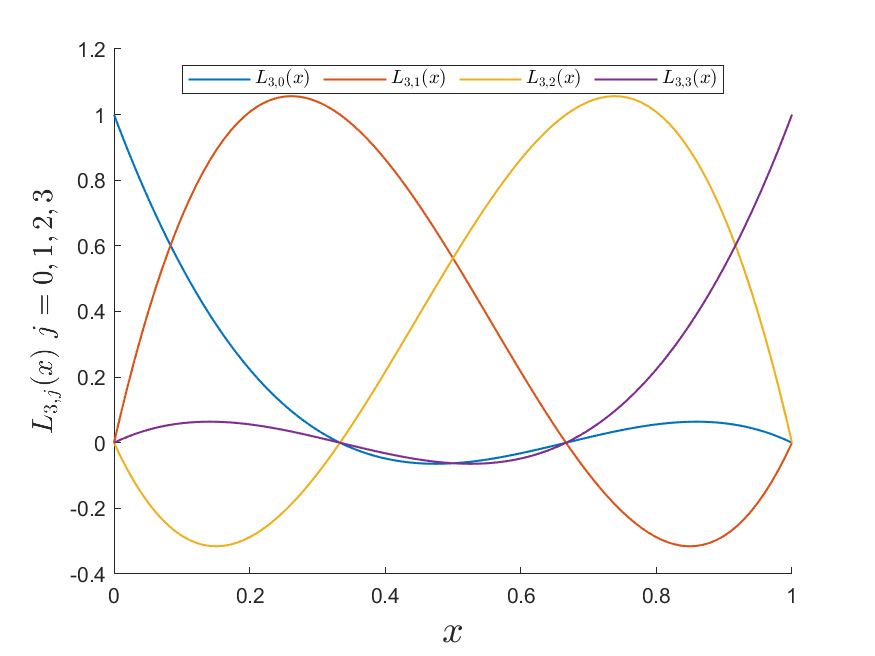
\includegraphics[width=150mm]{MATH391_Ass1_Fig2}}
\end{center}
{\bf Fig 1.} Degree 3 Lagrange polynomials, denoted $L_{3,j}(x)$ associated with four equidistant 
nodes $\{x_j\}_{1\leq j\leq 4}$ with $x_0<x_1<x_2<x_3$. In this example, $x_0=0$ and $x_3=1$.

\section*{Problem 3}
Let $n$ be a natural number and define
\[T_n(x)=\cos(n\arccos(x)),\indent -1\leq x\leq 1\]
to be the degree $n$ Chebeyshev polynomial. 

\subsection*{a) \normalfont Plot the graphs of $T_i(x)$, $i=1,2,3,4,5$.}
\begin{center}    
    \makebox[\textwidth]{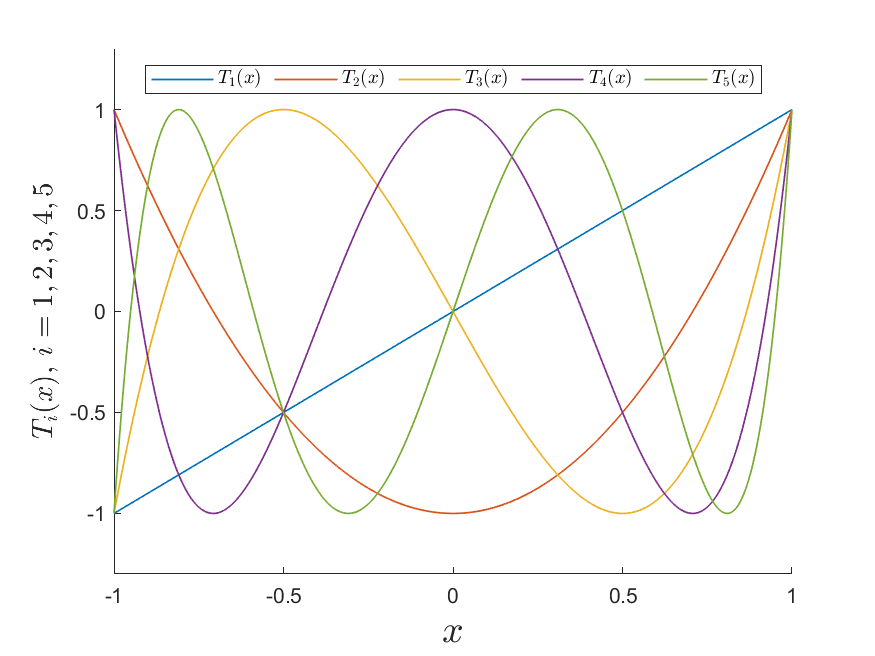
\includegraphics[width=150mm]{MATH391_Ass1_Fig3}}
\end{center}
{\bf Fig 2.} Degree $i$ Chebeyshev polynomials denoted $T_i(x)$ for $i=1,2,3,4,5$ over their domain
$-1\leq x\leq 1$. 

\subsection*{b) \normalfont Show that $T_n(x)$ is a polynomial of degree $n$.}
Let $n$ be a natural number. Then we begin with the trigonometric identity
\[\cos((n+1)\theta)+\cos((n-1)\theta)=2\cos(\theta)\cos(n\theta).\]
Now, let $\theta=\arccos(x)$. Then the above can be rewritten as
\begin{align*}
    \cos((n+1)\arccos(x))+\cos((n-1)\arccos(x))&=2\cos(\arccos(x))\cos(n\arccos(x))\\
    T_{n+1}(x)+T_{n-1}(x)&=2T_1(x)T_n(x).
\end{align*}
However, $T_1(x)=\cos(\arccos(x))=x$. From this we can easily construct the recurrence relation.
\begin{align*}
     T_{n+1}(x)+T_{n-1}(x)&=2xT_n(x)\\
     T_{n+1}(x)&=2xT_n(x)-T_{n-1}(x)\\
     T_{n}(x)&=2xT_{n-1}(x)-T_{n-2}(x) \text{\indent (shifting the indices.)}
\end{align*}
Where since $T_k(x)$ is defined for $k\in\mathbb{N}$, we require that $2\leq n$ for the recurrence
relation to hold. We proceed to use the recurrence relation to prove that $T_n(x)$ is a polynomial
of degree $n$. 

\begin{prf}[by induction]
    Let $n\in\mathbb{N}$ with $n\geq 2$ and $x\in\mathbb{R}$ with $-1\leq x\leq 1$. Then let $T_k(x)$ where $k\in\mathbb{N}$ be the degree $k$ 
    Chebeyshev polynomial defined by 
    \[T_k(x)=\cos(k\arccos(x))\]
    and $T_n(x)$ defined by the recurrence relation
    \[T_n(x)=2xT_{n-1}(x)-T_{n-2}(x).\]

    \noindent{\bf Basis}($k=0$, $k=1$). Suppose that $k=0$. Then we have that 
    \[T_k(x)=T_0(x)=\cos(0\arccos(x))=\cos(0)=1\]
    Where $T_0(x)=1$ is a polynomial of degree $0=k$.
    Next, suppose that $k=1$. Then we have that
    \[T_k(x)=T_1(x)=\cos(\arccos(x))=x\]
    Where $T_1(x)=x$ is a polynomial of degree $1=k$. Hence, in the base cases of $k=0$ and $k=1$,
    $T_k(x)$ is a polynomial of degree k.\\

    \noindent{\bf Inductive step.} Let $n\geq 2$ and suppose that for all $k\in\mathbb{N}$ where $0\leq k<n$
    we have that $T_k(x)$ is a polynomial of degree $k$ (inductive hypothesis). We want to show that
    $T_n(x)$ is a polynomial of degree $n$. Let $\deg()$ be the function which maps any polynomial to its degree. 
    We begin with the recurrence relation.
    \begin{align*}
        T_n(x)=2xT_{n-1}(x)-T_{n-2}(x)
    \end{align*}
    By the inductive hypothesis, we have that $T_{n-1}(x)$ is a polynomial of degree $n-1$ since $0\leq n-1<n$. 
    Furthermore, we have that $T_{n-2}(x)$ is a polynomial of degree $n-2$ since $0\leq n-2<n$. 
    Now we see that $2xT_{n-1}(x)$ is a polynomial of degree $n$, since $\deg(2x)=1$. However, for any two polynomials
    $P_a(x)$ and $P_b(x)$ where $\deg(P_a(x))=a$ and $\deg(P_b(x))=b$ with $a>b$, we have that $P_a(x)-P_b(x)$ is a polynomial and $\deg(P_a(x)-P_b(x))=a$. 
    Therefore since $\deg(2xT_{n-1}(x))=n$ and $\deg(T_{n-2}(x))=n-2$, we have that $\deg(2xT_{n-1}(x)-T_{n-2}(x))=n$,
    so $T_n(x)$ is a polynomial and $\deg(T_n(x))=n$.\\

    \noindent Now, by the base cases of $k=0$ and $k=1$, the inductive step and the principle of mathematical induction
    (strong form) we have that $T_n(x)$ is a polynomial of degree $n$ for all $n\in\mathbb{N}$.\indent\indent\indent\indent\indent\indent\indent\indent\indent\indent $\square$
\end{prf}

\subsection*{c) \normalfont Find the roots $\{\xi_i\}_{1\leq i\leq n}$ of $T_n(x)$.}
To begin, consider the definition of $T_n(x)$.
\[T_n(x)=\cos(n\arccos(x))\]
for $n\in\mathbb{N}$ and $x\in\mathbb{R}$, $-1\leq x\leq 1$. To find the roots, first let $\theta=n\arccos(x)$ 
so that we have $T_n(x)=\cos(\theta)$. Importantly, we have that $0\leq \theta\leq n\pi$. Then we rewrite $T_n(x)$.
\begin{align*}
    &T_n(x)=\cos(\theta)
\end{align*}
Letting $\theta_c$ be the possible values of $\theta$ for which $\cos(\theta)=0$, we have
\begin{align*}
    &\cos(\theta_c)=0\Rightarrow \theta_c=\pm\frac{\pi}{2},\pm\frac{3\pi}{2}, \pm\frac{5\pi}{2},\dots,\pm\frac{(2k-1)\pi}{2},\indent k\in\mathbb{Z}.
\end{align*}
However, since $\theta$ is bounded,  we need to enforce the appropriate bounds on $\theta_c$.
\[0\leq \theta_c\leq n\pi\Rightarrow 0\leq \frac{(2k-1)\pi}{2}\leq n\pi\Rightarrow \frac{1}{2}\leq k\leq n+\frac{1}{2}\Rightarrow k=1,2,3,...,n\text{\indent (since $k\in\mathbb{Z}$).}\]
Finally, we can determine the $n$ roots of $T_n(x)$, the $i^{th}$ of which we will denote $\xi_i$, $1\leq i\leq n$.
\begin{align*}
    n\arccos(\xi_i)&=\theta_c\\
    n\arccos(\xi_i)&=\frac{(2i-1)\pi}{2}\text{\indent (where $i=1,2,3,...,n$)}\\
    \arccos(\xi_i&=\frac{(2i-1)\pi}{2n}\\
    \xi_i&=\cos\left(\frac{(2i-1)\pi}{2n}\right)
\end{align*}
Where for $T_n(x)$ there are $n$ distinct values of $i$, so there are $i$ roots of the form
\[\xi_i=\cos\left(\frac{(2i-1)\pi}{2n}\right).\]

\subsection*{d) \normalfont Compute $\max_{-1\leq x\leq 1}|(x-\xi_1)(x-\xi_2)\dots(x-\xi_n)|$, where $\{\xi_i\}_{1\leq i\leq n}$ are the $n$ roots of $T_n(x)$.}
First, suppose that $-1\leq x\leq 1$. Clearly, $(x-\xi_1)(x-\xi_2)\dots(x-\xi_n)$ is a degree $n$ polynomial with the same roots as $T_n(x)$. 
This means that $(x-\xi_1)(x-\xi_2)\dots(x-\xi_n)=CT_n(x)$ for some constant $C$ so long as $n\neq 0$. Furthermore, we have that
\begin{align*}
    &\max_{-1\leq x\leq 1}|(x-\xi_1)(x-\xi_2)\dots(x-\xi_n)|=\max_{-1\leq x\leq 1}|CT_n(x)|\\
    &=C(1)\text{\indent (since $T_n(x)=\cos(n\arccos(x))$, so $-1\leq T_n(x)\leq 1$ and $|T_n(x)|\leq 1$).}
\end{align*}
Importantly, the leading coefficient of $(x-\xi_1)(x-\xi_2)\dots(x-\xi_n)$ is $1$, so if we suppose that $B$
is the leading coefficient of $T_n(x)$, then $C=B^{-1}$. We proceed by finding $B$. $T_{n=2}(x)$ is given by
\[T_{n=2}(x)=2x(x)-1=2x^2-1\]
which has leading coefficient $2=2^1=2^{n-1}$. By the recurrence relation, we can compute the next few Chebeyshev polynomials.
\begin{align*}
    T_{n=3}(x)&=2xT_2(x)-T_1(x)=4x^3-2x-x=4x^3-3x=2^2x^3-3x=2^{n-1}x^3-3x\\
    T_{n=4}(x)&=2xT_3(x)-T_2(x)=8x^4-6x^2-2x^2+1=8x^4-8x^2+1=2^3x^4-8x^2+1=2^{n-1}x^4-8x^2+1\\
    T_{n=5}(x)&=2xT_4(x)-T_3(x)=16x^5-16x^3+2x-4x^3+3x=16x^5-20x^3+5x=2^{n-1}x^5-20x^3+5x\\
    .\\
    .\\
    .
\end{align*}
So the leading coefficient of $T_n(x)$ appears to have the form $2^{n-1}$, which we will now endeavor to prove by 
induction. Taking the above to satisfy the base cases of $0<n\leq 5$, we proceed directly to the inductive step.\\

\noindent{\bf Inductive step.} Let $n\geq 6$ be a natural number and suppose that $\forall_k\in\mathbb{N}$, $1\leq k < n$ we have
that the leading coefficient of $T_k(x)$ is $2^{k-1}$ (inductive hypothesis). We want to show that
the leading coefficient of $T_n(x)$ is $2^{n-1}$. By the recurrence relation we have
\[T_n(x)=2xT_{n-1}(x)-T_{n-2}(x).\]
Now, since $1\leq n-1 < n$, the leading coefficient of $T_{n-1}(x)$ is $2^{n-2}$ by the inductive hypothesis. 
Note that this term is also the highest order among those in $T_{n-1}(x)-T_{n-2}(x)$. Let $2^{n-2}P_{n-1}(x)=T_{n-1}(x)$, where now
$P_{n-1}(x)$ is a degree $n-1$ polynomial with leading coefficient $1$. Then we have
\[2xT_{n-1}(x)=2x(2^{n-2}P_{n-1}(x))=2^{n-1}xP_{n-1}(x)\]
so $2xT_{n-1}(x)$ is a degree $n$ polynomial with leading coefficient $2^{n-1}$. Since this term is the highest order term
on the RHS of the recurrence relation, it is also the highest order term in $T_n(x)$, so the leading coefficient of $T_n(x)$ is
$2^{n-1}$.\\

\noindent By the base case of $0 < n\leq 5$, the inductive step and the principle of mathematical induction,
we have that the leading coefficient of the degree $n$ Chebeyshev polynomial (where $n>0$) is $2^{n-1}$. \indent\indent\indent\indent\indent\indent\indent\indent$\square$\\

\noindent As found above, letting $B$ be the leading coefficient of $T_n(x)$, we have that $B=2^{n-1}$. 
But $C=B^{-1}$, so $C=2^{1-n}=\frac{1}{2^{n-1}}$. Then we have that
\begin{align*}
    \max_{-1\leq x\leq 1}|(x-\xi_1)(x-\xi_2)\dots(x-\xi_n)|&=C\\
    &=\frac{1}{2^{n-1}}.
\end{align*}

\section*{Problem 4}

    \subsection*{a) \normalfont Plot the graphs of $f(x)$, $P_2(x)$, $P_4(x)$, $P_6(x)$, $P_8(x)$.}
    \begin{center}
        \makebox[\textwidth]{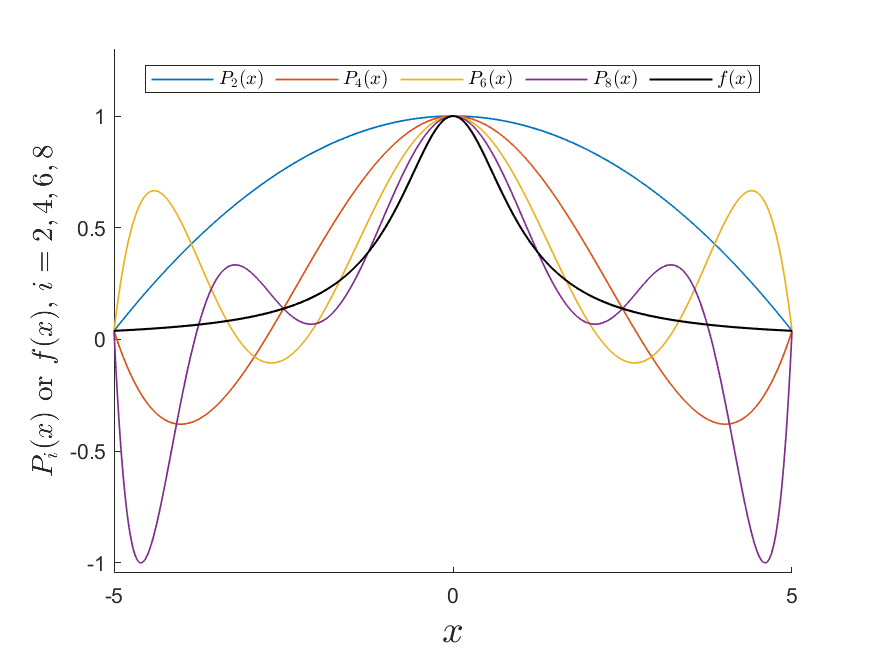
\includegraphics[width=150mm]{MATH391_Ass1_Fig4.png}}
    \end{center}
    {\bf Fig 3.} Function $f(x)=\frac{1}{1+x^2}$ plotted alongside degree $n$ interpolating polynomials $P_n(x)$ for 
    $n=2,4,6,8$. Here, $P_n(x)$ interpolates $n+1$ evenly spaced points defined by $\{(x_i, f(x_i))\}_{0\leq i\leq n}$
    where $x_i=-5+\frac{10i}{n}$.

    \subsection*{b) \normalfont Comment on the closeness of the interpolating polynomials to $f(x)$ around
    the middle and endpoints of $[-5,5]$.}
    Let $f(x)=\frac{1}{1+x^2}$. Then $f(x)$ has at least $10$ continuous derivatives on the interval $[-5,5]$,
    which contains the interpolatory points. Let $P_n(x)$ be the polynomial of degree $n$ interpolating $n+1$ linearly
    spaced nodes on $[-5,5]$. Then we have that
    \[f(x)-P_n(x)=\frac{f^{(n+1)}(\theta)}{(n+1)!}(x-x_0)(x-x_1)\dots(x-x_n)\]
    for some $\theta(x)\in[-5,5]$ for some $x\in[-5,5]$. In part {\bf a)} we considered the cases of $n=2,4,6,8$, so 
    we first consider the graphs of $f^{(n+1)}(x)$ on the interval $[-5,5]$ for these cases.
    \begin{center}
        \makebox[\textwidth]{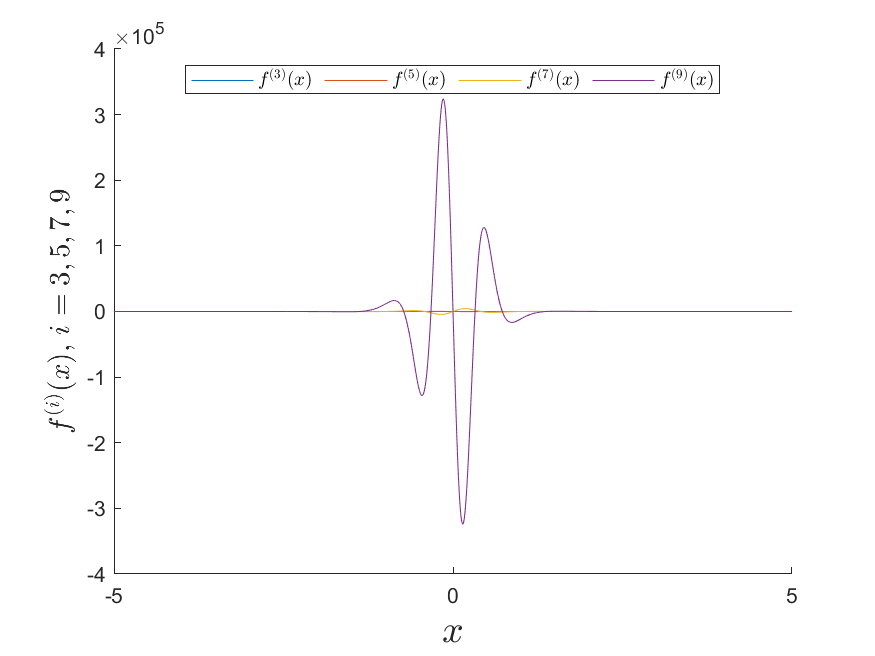
\includegraphics[width=150mm]{MATH391_Ass1_Fig5.png}}
    \end{center}
    {\bf Fig 4.} Graphs of $f^{(3)}(x)$, $f^{(5)}(x)$, $f^{(7)}(x)$, $f^{(9)}(x)$ for $x\in[-5,5]$.\\

    \noindent Where it is clear that $||f^{(9)}(x)||_{\infty}$ for $x\in[-5,5]$ dwarfs the other derivatives plotted, so 
    $f(x)-P_n(x)$ has the potential to be much higher for $n=9$ than $n<9$. This does not tell us where on the interval
    the error will be greatest since $\theta(x)$ is not known. Let $\omega_n(x)=(x-x_0)(x-x_1)\dots(x-x_n)$. Then for $x$ near
    either endpoint, with $x\neq x_0$ and $x\neq x_n$, $x$ is distant from all nodes except the endpoints, so the maxima of $\prod_{i=1}^{n-1}(x-x_i)$
    are maximized (multiplied by several numbers $>1$). Likewise, near the middle of the interval the maxima of the product 
    are not allowed to take great values, since nodes on either side of $x$ scale the product by smaller values. 
    To visualize this, consider the following figure depicting $\omega_n(x)$ for $n=2,4,6,8$ over interval $[-5,5]$.
    \begin{center}
        \makebox[\textwidth]{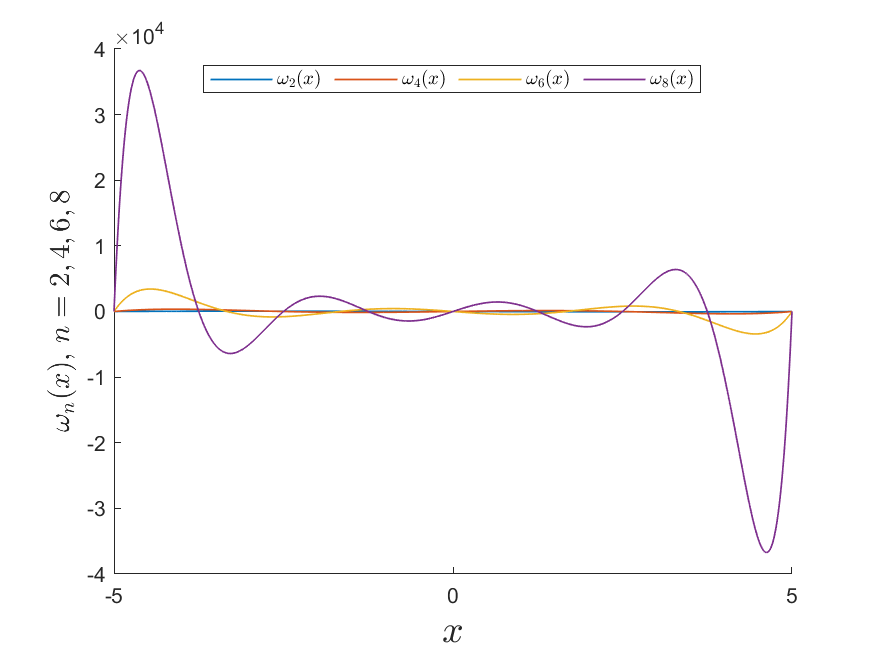
\includegraphics[width=105mm]{MATH391_Ass1_Fig6.png}}
    \end{center} 
    {\bf Fig 5.} Graphs of $\omega_2(x)$, $\omega_4(x)$, $\omega_6(x)$, $\omega_8(x)$ plotted for $x$ on interval
    $[-5,5]$. \\

    \noindent Here the phenomena described above is visualized, with $||\omega_n(x)||_{\infty}$ located near the endpoints. Furthermore,
    the maxima shown here are greater for increasing $n$.
    The consequence is that $f(x)-P_n(x)$ is highest near the endpoints as well, since only $\omega_n(x)$ has direct
    dependence on $x$ in $f(x)-P_n(x)=\frac{f^{(n+1)}(\theta(x))}{(n+1)!}\omega_n(x)$. 

\section*{Problem 5}
   Let $P_n(x)$ be the degree $n$ polynomial interpolating $f(x)$ at the $n+1$ pairwise distinct points 
   $X=\{x_0,\dots x_n\}$. Let $t\notin X$. Then let the degree $n+1$ polynomial interpolating $X\cup\{t\}$
   be given by $P_{n+1}(x)$. Then by the Newton form of the interpolating polynomials, we have that
   \begin{align*}
       &P_n(x)=a_0+a_1(x-x_0)+\dots+a_n(x-x_0)(x-x_1)\dots(x-x_{n-1})\\
       &P_{n+1}(x)=b_0+b_1(x-x_0)+\dots+b_n(x-x_0)(x-x_1)\dots(x-x_{n-1})+b_{n+1}(x-x_0)(x-x_1)\dots(x-x_n)
   \end{align*}
   Where $a_i$, $0\leq i \leq n$ are the $n+1$ real coefficients of $P_n(x)$ and similarly $b_j$, $0\leq j\leq n+1$
   are the $n+2$ real coefficients of $P_{n+1}(x)$. Then we have a theorem which allows us to assert that
   \begin{align*}
       a_i=f[x_0,\dots, x_i]=b_i
   \end{align*}
   where $f[x_0,\dots, x_i]$ is the $i^{th}$ divided difference for the nodes $X$ under $f$. This is true for all $0\leq i\leq n$.
   Hence we have that
   \begin{align*}
       &P_n(x)=f[x_0]+f[x_0,x_1](x-x_0)+\dots+f[x_0,x_1,\dots,x_n](x-x_0)(x-x_1)\dots(x-x_{n-1})\\
       &P_{n+1}(x)=f[x_0]+f[x_0,x_1](x-x_0)+\dots+f[x_0,x_1,\dots,x_n](x-x_0)(x-x_1)\dots(x-x_{n-1})\\
       &+f[x_0,x_1,\dots,x_n,t](x-x_0)(x-x_1)\dots(x-x_n)
   \end{align*}
   So from this we can see that
   \begin{align*}
       P_{n+1}(x)=P_n(x)+f[x_0,x_1,\dots,x_n,t](x-x_0)(x-x_1)\dots(x-x_n)
   \end{align*}
   Now, since $P_{n+1}(x)$ interpolates $f(x)$ at the nodes $X\cup\{t\}$, $P_{n+1}(t)=f(t)$, so we have that
   \begin{align*}
        f(t)=P_{n+1}(t)=P_n(t)+f[x_0,x_1,\dots,x_n,t](t-x_0)(t-x_1)\dots(t-x_n)
   \end{align*}
   as required.
\end{document}
